\documentclass[11pt]{article}
\usepackage[a4paper,margin=27mm]{geometry}
\usepackage{amsmath,amssymb,amsthm,mathtools}
\usepackage{booktabs}
\usepackage{graphicx}
\usepackage{float}
\usepackage{microtype}
\usepackage{xcolor}
\usepackage[hidelinks]{hyperref}
\usepackage{enumitem}

\newtheorem{theorem}{Theorem}[section]
\newtheorem{proposition}[theorem]{Proposition}
\newtheorem{corollary}[theorem]{Corollary}
\newtheorem{lemma}[theorem]{Lemma}
\newtheorem{remark}[theorem]{Remark}
\newcommand{\E}{\mathbb E}
\newcommand{\R}{\mathbb R}
\newcommand{\I}{\mathrm I}
\newcommand{\tr}{\operatorname{tr}}
\newcommand{\diag}{\operatorname{diag}}
\newcommand{\sech}{\operatorname{sech}}
\hypersetup{
 pdftitle={The Schwarzian Bridge in a Single Sigmoid Neuron},
 pdfauthor={Lluis Eriksson},
 pdfkeywords={single neuron, sigmoid, Loewner matrix, matrix monotonicity, Fisher information, saturation}
}

\title{\bfseries The Schwarzian Bridge in a Single Sigmoid Neuron\\
\large Exact L\"owner Determinants and Gaussian Saturation Anisotropy}
\author{Lluis Eriksson\\Independent Researcher\\\texttt{lluiseriksson@gmail.com}}
\date{August 2026}

\begin{document}
\maketitle

\begin{abstract}
A sigmoid is increasing on scalars, yet its bend controls two different geometries.  The classical Schwarzian
criterion implies that a negative-Schwarzian activation is not matrix-monotone of order two.  We give a closed
logistic formula showing every distinct two-point L\"owner determinant to be negative, a dimension-minimal
$2\times2$ positive-semidefinite perturbation witness certified with interval arithmetic, and the corresponding
classical serial-chain consequence.

Our central link is that the same local invariant determines the leading quadratic onset coefficient of saturation
anisotropy.  At a centered
inflection of an increasing activation $g$, for a sensitivity $h_p=(g')^p$,
\[
 \frac{\E h_p(rZ)}{\E[Z^2h_p(rZ)]}=1-p\,Sg(0)r^2+O(r^4),
\]
whereas the adjacent-point L\"owner determinant is
$g'(0)^2Sg(0)\delta^2/6+O(\delta^3)$.  Negative Schwarzian therefore simultaneously gives local
noncommutative order failure and positive initial radial--tangential anisotropy.

For isotropic Gaussian inputs in dimension $d\ge2$, population curvature at a teacher of norm $r$ has one radial eigenvalue and $d-1$ equal
tangential eigenvalues.  For any nonnegative sensitivity profile $h$ with finite defining expectations, these
eigenvalues are exactly
\[
 \alpha_h(r)=\E h(rZ),\qquad \beta_h(r)=\E[Z^2h(rZ)],\qquad Z\sim N(0,1),
\]
and, if its zeroth and second Lebesgue moments are finite and positive,
\[
 \alpha_h(r)\sim \frac{\varphi(0)m_0}{r},\qquad
 \beta_h(r)\sim \frac{\varphi(0)m_2}{r^3}.
\]
Thus saturation suppresses magnitude information by two additional powers: the radial--tangential ratio obeys
$\alpha_h(r)/\beta_h(r)\sim(m_0/m_2)r^2$.  For the logistic sigmoid this ratio is the spectral condition number,
and we evaluate its constants in closed form.  Squared-output
loss gives $\kappa(r)\sim 3r^2/(\pi^2-6)$, while Bernoulli likelihood gives
$\kappa(r)\sim3r^2/\pi^2$.  Prior work contains the Bernoulli exponents and the one-unit squared-output spectral
reduction; our additions are the Schwarzian bridge, profile-generic brackets, exact logistic constants, and strict
ratio monotonicity.  In both cases the anisotropy is strictly increasing from one.  We prove explicit finite-$r$
brackets, translate the law into optimally tuned stationary fixed-step local gradient-descent rates and
Cram\'er--Rao lower bounds, and supply a
deterministic replay.  The bridge identifies a shared local source for two effects already present in one neuron,
while the large-$r$ theorem quantifies the later saturation regime.
\end{abstract}

\paragraph{Keywords.} single neuron; sigmoid; matrix monotonicity; L\"owner order; Schwarzian derivative;
Fisher information; Gaussian design.

\section{Question, result, and claim boundary}

The scalar logistic curve is
\[
 \sigma(s)=\frac1{1+e^{-s}},\qquad
 \sigma'(s)=\frac1{4}\sech^2(s/2).
\]
It is strictly increasing, so larger scalar scores produce larger outputs.  We first ask whether this order survives
spectral functional calculus on noncommuting matrices.  It does not, at the smallest possible matrix size and on
every interval.  We then return to the ordinary teacher neuron $\sigma(w_\star^\top X)$ with
$X\sim N(0,I_d)$.  There, a perturbation perpendicular to $w_\star$ rotates the separating hyperplane, while a
parallel perturbation changes its confidence scale and must be detected through samples near the transition layer.
Our goal is to compute both failures exactly.

The main contributions are:
\begin{enumerate}[leftmargin=2em]
 \item a closed logistic specialization of the classical negative-Schwarzian obstruction, proving directly that
 every nontrivial two-point L\"owner matrix is indefinite;
 \item a dimension-minimal $2\times2$ witness $A\preceq B$ but $\sigma(A)\npreceq\sigma(B)$, with
 outward-rounded eigenvalue certification, and a L\"owner-order reformulation of the known serial-composition
 consequence;
 \item a Schwarzian bridge equating the local order defect with the leading radial--tangential anisotropy of the
 Gaussian sensitivity matrix at a centered inflection;
 \item a profile-generic two-eigenvalue refinement under Gaussian design, with source-level finite-$r$ brackets,
 closed logistic constants and strict ratio monotonicity for both $h=\sigma'$ and $h=\sigma'^2$; and
 \item exact local consequences for stationary fixed-step optimization and estimation, plus a one-command replay
 of the identities,
 interval witness, inequalities, and figure.
\end{enumerate}

The matrix-order theorem concerns spectral functional calculus $\sigma(A)$, not entrywise activation of a vector.
The radial theorem is not a claim about deep networks, global optimization, implicit bias, or arbitrary inputs.  The
two questions meet at a precise boundary: scalar monotonicity controls neither noncommuting PSD perturbations nor
the conditioning of parameter directions.

\section{A sigmoid is not an order-preserving operator}

For Hermitian matrices, $A\preceq B$ means that $B-A$ is positive semidefinite.  A scalar function $f$ is
\emph{matrix-monotone of order two} on an interval $J$ if $f(A)\preceq f(B)$ for every pair of $2\times2$
Hermitian matrices with spectra in $J$ and $A\preceq B$, where $f(A)$ is defined by spectral functional calculus.
If $A$ and $B$ commute, scalar monotonicity is sufficient because they are simultaneously diagonalizable.  The
question is what happens without commutativity.

For distinct $x,y\in J$, define the two-point L\"owner matrix
\begin{equation}
 L_f(x,y)=
 \begin{pmatrix}
  f'(x)&\dfrac{f(x)-f(y)}{x-y}\\[5pt]
  \dfrac{f(x)-f(y)}{x-y}&f'(y)
 \end{pmatrix}.
 \label{eq:loewnermatrix}
\end{equation}
The fixed-order L\"owner criterion says that matrix monotonicity of order two requires
$L_f(x,y)\succeq0$ for every pair \cite{hiai2010,heinavaara2019}.  The equivalent local criterion
$Sf\ge0$ for increasing smooth functions is classical \cite[Lemma 10]{kozlovski2008}; the result below is an
explicit logistic specialization, not a new qualitative matrix-monotonicity criterion.

Cook, Hammerlindl and Tucker define
\[
 \chi_f(x,y)=f'(x)f'(y)
 \left(\frac{x-y}{f(x)-f(y)}\right)^2
\]
and study the class $\chi_f\le1$, including sigmoid activations and serial compositions \cite{cook2023}.  If
$D_f(x,y)=(f(x)-f(y))/(x-y)$, then
\begin{equation}
 \det L_f(x,y)=D_f(x,y)^2\,[\chi_f(x,y)-1].
 \label{eq:coexpanding}
\end{equation}
Thus their two-point inequality is algebraically the nonpositive L\"owner-determinant inequality.  Our contribution
in this subsection is the strict closed logistic identity and the certified matrix witness, not the underlying
Schwarzian/composition mechanism.

\begin{theorem}[closed logistic two-point determinant]
\label{thm:loewner}
Let
\[
 s_{\alpha,b}(x)=\frac1{1+e^{-\alpha(x-b)}},\qquad \alpha>0.
\]
For every $x\ne y$, the L\"owner matrix $L_{s_{\alpha,b}}(x,y)$ has negative determinant.  Consequently the
logistic activation is not matrix-monotone of order two on any nondegenerate interval.
\end{theorem}

\begin{proof}
Put $u=e^{\alpha(x-b)}$, $v=e^{\alpha(y-b)}$, and $r=v/u=e^{\alpha(y-x)}$.  Direct cancellation gives the exact
identity
\begin{equation}
 \det L_{s_{\alpha,b}}(x,y)
 =\frac{\alpha^2u^2}{(1+u)^2(1+v)^2}
 \left[r-\frac{(r-1)^2}{(\log r)^2}\right].
 \label{eq:loewnerdet}
\end{equation}
For $r\ne1$, write $t=\log r$.  Strict convexity of $\sinh$ on $(0,\infty)$ gives
\[
 |r-1|=2e^{t/2}|\sinh(t/2)|>e^{t/2}|t|=\sqrt r\,|\log r|.
\]
The bracket in \eqref{eq:loewnerdet} is therefore strictly negative.  Every nondegenerate interval contains a
distinct pair, so the L\"owner criterion completes the proof.
\end{proof}

This is stronger than finding one bad scale: changing the slope $\alpha$, shifting the bias $b$, or restricting the
score range never removes the obstruction.  It also identifies the precise failure.  The diagonal entries in
\eqref{eq:loewnermatrix} are positive, but the divided difference is too large for their geometric mean.

\begin{proposition}[dimension-minimal explicit PSD witness]
\label{prop:witness}
For the standard logistic sigmoid, let
\begin{equation}
 A=\begin{pmatrix}-1/2&0\\0&1/2\end{pmatrix},\qquad
 B=A+\frac1{100}\begin{pmatrix}1&1\\1&1\end{pmatrix}.
 \label{eq:witness}
\end{equation}
Then $A\preceq B$ but $\sigma(A)\npreceq\sigma(B)$.  At 256-bit outward-rounded Arb precision,
\begin{align}
 \operatorname{spec}(B)&\subset[-0.4901000,-0.4900999]\cup[0.5100999,0.5101000],\\
 \operatorname{spec}(\sigma(B)-\sigma(A))
 &\subset[-9.9150,-9.9147]\,10^{-5}\ \cup\ [0.0047990,0.0047992],\label{eq:witnessspec}\\
 \det(\sigma(B)-\sigma(A))&\in[-4.7583,-4.7581]\,10^{-7}.
\end{align}
\end{proposition}

\begin{proof}
$B-A$ has eigenvalues $0$ and $1/50$.  If $a=1/2$, $\varepsilon=1/100$, and
$d=(a^2+\varepsilon^2)^{1/2}$, then $B$ has eigenvalues $\lambda_\pm=\varepsilon\pm d$ and
\[
 \sigma(B)=mI+n(B-\varepsilon I),\quad
 m=\frac{\sigma(\lambda_+)+\sigma(\lambda_-)}2,\quad
 n=\frac{\sigma(\lambda_+)-\sigma(\lambda_-)}{2d}.
\]
Substitution reduces the three enclosures to scalar exponential and square-root balls.  The replay evaluates them
with directed Arb rounding; the negative eigenvalue in \eqref{eq:witnessspec} proves the claim.
\end{proof}

The witness is illustrative, while Theorem~\ref{thm:loewner} is the proof for every interval.  The derivative form
also explains why an indefinite L\"owner matrix produces witnesses: for diagonal
$A=\diag(x,y)$, the Fr\'echet derivative in the all-ones PSD direction is precisely the Schur product with
$L_f(x,y)$.

\subsection{Serial depth does not repair the order}

For a $C^3$ function with nonzero derivative, its Schwarzian is
\begin{equation}
 Sf=\frac{f'''}{f'}-\frac32\left(\frac{f''}{f'}\right)^2.
 \label{eq:schwarzian}
\end{equation}
The logistic sigmoid and a scaled hyperbolic tangent satisfy
\begin{equation}
 S s_{\alpha,b}=-\frac{\alpha^2}{2},\qquad
 S\tanh(\alpha x+\beta)=-2\alpha^2.
 \label{eq:schwarzianvalues}
\end{equation}

\begin{corollary}[serial spectral reformulation]
\label{thm:serial}
Let $F$ be a finite scalar composition of positive-slope affine maps and at least one increasing logistic or
hyperbolic-tangent activation.  Then $SF<0$ everywhere, and $F$ is not matrix-monotone of order two on any
nondegenerate interval.
\end{corollary}

\begin{proof}
The composition identity
\begin{equation}
 S(f\circ g)=(Sf\circ g)(g')^2+Sg
 \label{eq:schwarzchain}
\end{equation}
and \eqref{eq:schwarzianvalues} give $SF<0$, since positive affine maps have zero Schwarzian and all derivatives in
the chain are positive.  For $h\to0$, Taylor expansion of the two-point determinant gives
\begin{equation}
 \det L_F(x,x+h)=\frac{F'(x)^2}{6}\,SF(x)\,h^2+O(h^3).
 \label{eq:localschwarz}
\end{equation}
It is negative for all sufficiently small nonzero $h$.  Every interval contains such a pair.
\end{proof}

The corollary restates, in spectral L\"owner order, the serial closure proved in the nowhere-coexpanding framework
\cite{cook2023}.  It is deliberately about \emph{serial scalar chains}.  It does not cover sums of neurons, skip
connections, multivariate architectures, or entrywise coordinate order.  Its content is that composing more of the
same S-shaped bend cannot turn the resulting scalar function into a PSD-order-preserving spectral activation.

\section{Two models, one sensitivity matrix}

Write $r=\lVert w_\star\rVert$ and $u=w_\star/r$ when $r>0$.  We use two standard observation models.

\paragraph{Squared-output regression.}
For the realizable population loss
\begin{equation}
 \mathcal L_{\rm sq}(w)=\frac12\E\bigl[\sigma(w^\top X)-\sigma(w_\star^\top X)\bigr]^2,
 \label{eq:squareloss}
\end{equation}
the residual vanishes at $w_\star$, so its Hessian is the Gauss--Newton matrix
\begin{equation}
 H_{\rm sq}(w_\star)=\E\bigl[\sigma'(w_\star^\top X)^2XX^\top\bigr].
 \label{eq:squarehess}
\end{equation}
The same matrix, divided by a known output-noise variance $\tau^2$, is the Fisher information of
$Y=\sigma(w_\star^\top X)+\varepsilon$, $\varepsilon\sim N(0,\tau^2)$.

\paragraph{Bernoulli logistic neuron.}
If $Y\mid X\sim\mathrm{Bernoulli}(\sigma(w_\star^\top X))$, the expected negative-log-likelihood Hessian and the
Fisher information coincide:
\begin{equation}
 H_{\rm B}(w_\star)=\E\bigl[\sigma'(w_\star^\top X)XX^\top\bigr].
 \label{eq:bernhess}
\end{equation}

Both are instances of the sensitivity matrix
\begin{equation}
 H_h(r,u):=\E\bigl[h(r u^\top X)XX^\top\bigr], \qquad h\ge0.
 \label{eq:profilematrix}
\end{equation}
The power of the reduction below is that no high-dimensional integration remains.

Amari, Karakida and Oizumi already derived the exact one-unit Gaussian Fisher decomposition for
$h=\phi'^2$, including the radial--tangential split and the bias block \cite{amari2019}.  We do not claim that
decomposition or the squared-output branch as new.
For the Bernoulli profile $h=\sigma'$, Chen and Mazumdar recently identified the same radial and orthogonal
Hessian functions and proved their $r^{-3}$ and $r^{-1}$ orders in a finite-sample analysis of logistic regression
\cite{chen2026gd}.  Their follow-up proves the minimax norm-estimation rate $\Theta(\sqrt{r^3/n})$
\cite{chen2026minimax}.  We do not claim those exponents or the Bernoulli optimization penalty as new.  The
purpose of the next sections is to isolate the profile-generic mechanism, give finite-radius brackets and exact
logistic constants, prove strict monotonicity of both eigenvalue ratios, and connect their small-$r$ coefficients to
the Schwarzian order defect.

\section{Universal Gaussian saturation theorem}

Let $\varphi(z)=(2\pi)^{-1/2}e^{-z^2/2}$ and define the even sensitivity moments
\[
 m_j(h):=\int_{\R} t^j h(t)\,dt\quad(j=0,2,4),
\]
whenever finite.  Evenness of $h$ is not needed for the spectral reduction or leading asymptotics, but it holds in
our sigmoid applications and makes the interpretation symmetric.

\begin{theorem}[exact spectrum and finite-$r$ brackets]
\label{thm:universal}
Let $d\ge2$, $X\sim N(0,I_d)$, $r>0$, $u\in S^{d-1}$, and let $h:\R\to[0,\infty)$ be measurable with
$\E[(1+Z^2)h(rZ)]<\infty$.  Then
\begin{equation}
 H_h(r,u)=\alpha_h(r)(I-uu^\top)+\beta_h(r)uu^\top,
 \label{eq:decomp}
\end{equation}
where
\begin{equation}
 \alpha_h(r)=\E h(rZ),\qquad \beta_h(r)=\E[Z^2h(rZ)],\qquad Z\sim N(0,1).
 \label{eq:alphabeta}
\end{equation}
If $m_0,m_2<\infty$ and are positive, then
\begin{equation}
 \alpha_h(r)\sim\frac{\varphi(0)m_0}{r},\qquad
 \beta_h(r)\sim\frac{\varphi(0)m_2}{r^3},\qquad
 \kappa_h(r):=\frac{\alpha_h(r)}{\beta_h(r)}\sim\frac{m_0}{m_2}r^2.
 \label{eq:univasymp}
\end{equation}
If $m_0,m_2,m_4<\infty$, the following nonasymptotic brackets hold for every $r>0$:
\begin{align}
 \frac{\varphi(0)}r\left(m_0-\frac{m_2}{2r^2}\right)
 &\le \alpha_h(r)\le \frac{\varphi(0)m_0}{r},\label{eq:alphabounds}\\
 \frac{\varphi(0)}{r^3}\left(m_2-\frac{m_4}{2r^2}\right)
 &\le \beta_h(r)\le \frac{\varphi(0)m_2}{r^3}.
 \label{eq:betabounds}
\end{align}
Negative lower endpoints are interpreted as valid but uninformative bounds.
\end{theorem}

\begin{proof}
Decompose $X=Zu+Y$, where $Z\sim N(0,1)$, $Y\sim N(0,I-uu^\top)$, and $Z,Y$ are independent.
The mixed terms vanish and $\E YY^\top=I-uu^\top$, giving \eqref{eq:decomp}--\eqref{eq:alphabeta}.
Changing variables $t=rz$ gives the exact one-dimensional formulae
\begin{equation}
 \alpha_h(r)=\frac{\varphi(0)}r\int_\R h(t)e^{-t^2/(2r^2)}dt,
 \quad
 \beta_h(r)=\frac{\varphi(0)}{r^3}\int_\R t^2h(t)e^{-t^2/(2r^2)}dt.
 \label{eq:scaledintegrals}
\end{equation}
Dominated convergence proves \eqref{eq:univasymp}.  Finally,
$1-x\le e^{-x}\le1$ for $x\ge0$ inserted into \eqref{eq:scaledintegrals} proves
\eqref{eq:alphabounds}--\eqref{eq:betabounds}.
\end{proof}

\section{The Schwarzian bridge}

The matrix-order and saturation calculations meet exactly at an inflection point.  The next statement applies
beyond the logistic curve and turns that meeting into a coefficient identity.

\begin{theorem}[local order--anisotropy bridge]
\label{thm:bridge}
Let $g\in C^5(\R)$ satisfy $g'>0$ and $g''(0)=0$.  For $p>0$, suppose
$h_p=(g')^p$ is $C^4$ with bounded fourth derivative, and define
\[
 \alpha_p(r)=\E h_p(rZ),\qquad \beta_p(r)=\E[Z^2h_p(rZ)],\qquad
 \kappa_p(r)=\frac{\alpha_p(r)}{\beta_p(r)}.
\]
Then
\begin{equation}
 \lim_{r\downarrow0}\frac{\kappa_p(r)-1}{r^2}
 =-p\,Sg(0)
 =-\frac{6p}{g'(0)^2}
   \lim_{\delta\to0}\frac{\det L_g(0,\delta)}{\delta^2}.
 \label{eq:bridge}
\end{equation}
In particular, $Sg(0)<0$ makes $L_g(0,\delta)$ indefinite for every sufficiently small
$\delta\ne0$ and makes $\kappa_p(r)>1$ for all sufficiently small $r>0$.
\end{theorem}

\begin{proof}
Taylor expansion under the Gaussian expectation, with the bounded fourth derivative controlling the remainder,
gives
\[
 \alpha_p(r)=h_p(0)+\frac{h_p''(0)}2r^2+O(r^4),\qquad
 \beta_p(r)=h_p(0)+\frac{3h_p''(0)}2r^2+O(r^4).
\]
Consequently
\[
 \kappa_p(r)=1-\frac{h_p''(0)}{h_p(0)}r^2+O(r^4).
\]
Because $\log h_p=p\log g'$ and $g''(0)=0$,
\[
 \frac{h_p''(0)}{h_p(0)}
 =p\frac{g'''(0)}{g'(0)}
 =p\,Sg(0).
\]
Finally, the adjacent-point expansion \eqref{eq:localschwarz}, applied to $g$ at zero, yields the second equality
in \eqref{eq:bridge}.
\end{proof}

For the standard logistic sigmoid, $S\sigma=-1/2$.  Theorem~\ref{thm:bridge} therefore predicts the exact initial
coefficients $1/2$ for $h_1=\sigma'$ and $1$ for $h_2=\sigma'^2$, recovered globally below in
\eqref{eq:smallbern}--\eqref{eq:smallsq}.  This equality of coefficients is the promised bridge: it does not merely
place two sigmoid facts side by side, but identifies their common differential invariant.

For a general $h$, $\kappa_h=\alpha_h/\beta_h$ in \eqref{eq:univasymp} is an anisotropy ratio; it is the spectral
condition number only after the eigenvalue ordering is known.  The two powers are geometric.  At large $r$, only a
score slab of width $O(r^{-1})$ remains unsaturated, producing
$\alpha\asymp r^{-1}$.  A radial perturbation carries an additional factor $Z^2=O(r^{-2})$ inside that slab,
producing $\beta\asymp r^{-3}$.  Both modes are supported by the near-boundary slab; the radial mode is weaker
because it carries the additional $Z^2$ factor.

\section{The logistic constants and the exact saturation profile}

For $p\in\{1,2\}$ set $h_p(t)=\sigma'(t)^p$.  The case $p=1$ is Bernoulli Fisher curvature and $p=2$ is
squared-output curvature.

\begin{lemma}[closed sensitivity moments]
\label{lem:moments}
The first three even moments are
\begin{center}
\begin{tabular}{c@{\qquad}ccc}
\toprule
profile & $m_0$ & $m_2$ & $m_4$\\
\midrule
$h_1=\sigma'$ & $1$ & $\pi^2/3$ & $7\pi^4/15$\\[2pt]
$h_2=\sigma'^2$ & $1/6$ & $(\pi^2-6)/18$ & $7\pi^4/90-2\pi^2/3$\\
\bottomrule
\end{tabular}
\end{center}
\end{lemma}

\begin{proof}
For $h_1$, these are the normalization, variance, and fourth central moment of the standard logistic density.
For $h_2(t)=\frac1{16}\sech^4(t/2)$, its Fourier transform is
\begin{equation}
 \widehat h_2(k)=\int_\R e^{ikt}h_2(t)dt
 =\frac16\,\Gamma(2+ik)\Gamma(2-ik).
 \label{eq:fourier}
\end{equation}
Differentiating at zero and using
$\psi_1(2)=\pi^2/6-1$ and $\psi_3(2)=\pi^4/15-6$ gives the displayed values.
\end{proof}

\begin{theorem}[strict logistic anisotropy]
\label{thm:monotone}
For $p=1$ and $p=2$, $\kappa_p(0)=1$, $\kappa_p(r)>1$ for $r>0$, and $\kappa_p$ is strictly increasing on
$(0,\infty)$.  Moreover,
\begin{equation}
 \kappa_1(r)\sim\frac{3}{\pi^2}r^2,
 \qquad
 \kappa_2(r)\sim\frac{3}{\pi^2-6}r^2.
 \label{eq:logisticconstants}
\end{equation}
\end{theorem}

\begin{proof}
Normalize the density $q_{p,r}(z)\propto h_p(rz)\varphi(z)$.  Then
$\beta_p(r)/\alpha_p(r)=\E_{q_{p,r}}Z^2$.  If $r_2>r_1$, the derivative on $z>0$ of the log likelihood ratio is
\[
 \frac d{dz}\log\frac{h_p(r_2z)}{h_p(r_1z)}
 =-p\bigl[r_2\tanh(r_2z/2)-r_1\tanh(r_1z/2)\bigr]<0.
\]
Thus the distribution of $|Z|$ under $q_{p,r}$ decreases strictly in monotone-likelihood-ratio order as $r$
increases, and its strictly increasing statistic $Z^2$ has decreasing expectation.  Hence $\alpha_p/\beta_p$
increases strictly.  At $r=0$ isotropy gives one, and Lemma~\ref{lem:moments} inserted into
Theorem~\ref{thm:universal} gives \eqref{eq:logisticconstants}.
\end{proof}

Figure~\ref{fig:saturation} shows the entire saturation profile.  The solid and dashed curves are direct Gaussian
integrals; the dotted curves are the asymptotic constants in \eqref{eq:logisticconstants}.

\begin{figure}[H]
 \centering
 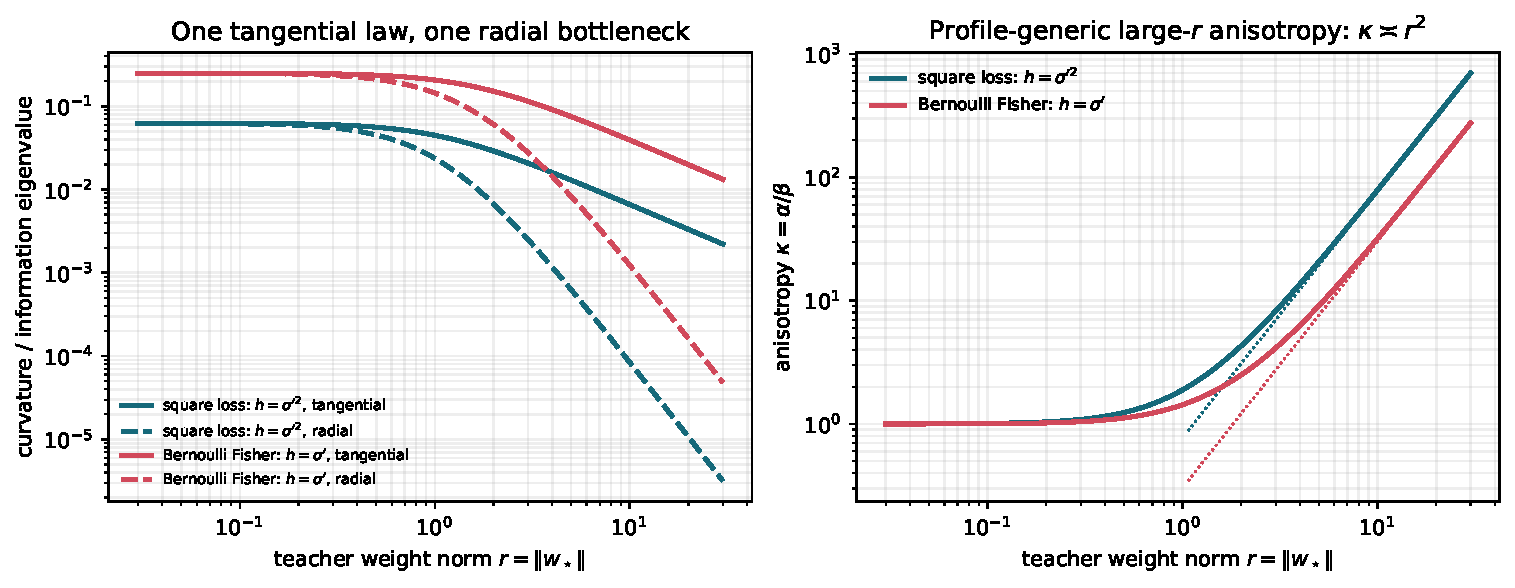
\includegraphics[width=\textwidth]{../figures/saturation_law.pdf}
 \caption{Exact curvature/information eigenvalues and their ratio.  Saturation leaves $d-1$ tangential directions
 at order $r^{-1}$ but pushes the radial direction to order $r^{-3}$.  The quadratic condition-number law is not a
 fitted exponent; it follows from Theorem~\ref{thm:universal}.}
 \label{fig:saturation}
\end{figure}

At the nonsaturated endpoint the expansions are also explicit:
\begin{align}
 \kappa_1(r)&=1+\tfrac12r^2-\tfrac18r^4+O(r^6),\label{eq:smallbern}\\
 \kappa_2(r)&=1+r^2-\tfrac14r^4+O(r^6).\label{eq:smallsq}
\end{align}
They follow by expanding $\sech^2(rZ/2)$ and $\sech^4(rZ/2)$ and using Gaussian moments.

\section{What the law costs}

\subsection{Stationary fixed-step gradient descent}

For either logistic profile, assume $d\ge2$ and that one constant scalar step size $\eta$ is reused at every
iteration.  At the teacher, the
Jacobian of one gradient-descent step is $I-\eta H_h$.  Its radial eigenvalue is
$1-\eta\beta$ and its tangential eigenvalue is $1-\eta\alpha$.  The best scalar step for this local quadratic model is
\begin{equation}
 \eta_\star=\frac{2}{\alpha+\beta},\qquad
 \rho_\star=\frac{\alpha-\beta}{\alpha+\beta}=\frac{\kappa-1}{\kappa+1}.
 \label{eq:optrate}
\end{equation}
Consequently $-\log\rho_\star\sim2/\kappa$.  For worst-case local error with components allowed in both
eigenspaces, the e-folding iteration count
$T_{\rm e}:=(-\log\rho_\star)^{-1}$ therefore has the exact leading scaling
\begin{equation}
 T_{{\rm e},\rm sq}\sim\frac{3}{2(\pi^2-6)}r^2,\qquad
 T_{{\rm e},\rm B}\sim\frac3{2\pi^2}r^2
 \label{eq:iterationtax}
\end{equation}
for the optimally tuned stationary scalar-step linearization.  This is not a global iteration bound or an
algorithm-independent obstruction: away from the teacher the Hessian contains residual terms, and nonstationary
polynomial methods can exploit the two-point spectrum.  Indeed, the scalar schedule
$\eta_1=1/\alpha$, $\eta_2=1/\beta$ makes
$(I-\eta_2H)(I-\eta_1H)=0$ in this exact local quadratic.  Natural-gradient or matrix-preconditioned updates can
also remove the local condition number by acting differently on the two eigenspaces.

\subsection{Estimation}

For $n$ independent Gaussian-output observations with known variance $\tau^2$, the Fisher information is
$nH_{h_2}/\tau^2$.  The Cram\'er--Rao inequality gives, along any unit tangential vector $v\perp u$ and the radial
vector $u$,
\begin{equation}
 \operatorname{Var}(v^\top\widehat w)\ge\frac{\tau^2}{n\alpha_2(r)},\qquad
 \operatorname{Var}(u^\top\widehat w)\ge\frac{\tau^2}{n\beta_2(r)}.
 \label{eq:crgauss}
\end{equation}
The ratio of the displayed radial lower bound to the tangential lower bound is $\kappa_2(r)$.  Hence tangential
variance is bounded below at order $r/n$, while radial variance is bounded below at order
$r^3/n$.  The analogous Bernoulli bounds replace $h_2$ by $h_1$.  The same quadratic ratio therefore appears in
these coordinatewise information lower bounds and in stationary fixed-step descent, although the latter can be
removed by a nonstationary schedule.

\section{Bias and universality}

A conventional neuron includes a bias $b$.  At $b=0$ the augmented parameter $(w,b)$ has Fisher/Hessian block
\[
 \E\!\left[h(rZ)
 \begin{pmatrix}XX^\top&X\\X^\top&1\end{pmatrix}\right].
\]
For even $h$, the radial--bias cross term $\E[Zh(rZ)]$ vanishes.  The bias eigenvalue equals $\alpha_h(r)$, so
the spectrum contains one radial eigenvalue $\beta_h$ and $d$ tangential/bias eigenvalues $\alpha_h$.  A nonzero
bias preserves the $(d-1)$ tangential eigenspace but replaces the radial and bias coordinates by the explicit
$2\times2$ block
\begin{equation}
 \begin{pmatrix}
  \E[Z^2h(rZ+b)] & \E[Zh(rZ+b)]\\
  \E[Zh(rZ+b)] & \E[h(rZ+b)]
 \end{pmatrix}.
 \label{eq:biasblock}
\end{equation}
The centered theorem is therefore not an artifact of omitting the bias; it is the diagonal point of a fully explicit
two-coordinate extension.

The exponent two is broader than the logistic curve.  Theorem~\ref{thm:universal} shows that any localized
sensitivity profile with finite positive $m_0$ and $m_2$ has the same $r^2$ anisotropy, with only the constant
$m_0/m_2$ depending on the activation and observation model.  Profiles with heavy sensitivity tails or vanishing
second moment fall outside this universality class and can have different laws.

\section{Relation to prior work}

L\"owner matrices characterize fixed-order matrix monotonicity; modern treatments include Hiai--Sano and
Hein\"avaara \cite{hiai2010,heinavaara2019}.  Kozlovski and Sands prove the relevant classical equivalence between
$Sf\ge0$ and order-two matrix monotonicity and record the Schwarzian composition law
\cite{kozlovski2008}.  Hence the qualitative logistic obstruction and its serial-chain extension are classical
consequences; negative Schwarzian also implies the all-pair determinant sign through strict convexity of
$(f')^{-1/2}$.  Cook, Hammerlindl and Tucker develop the algebraically equivalent nowhere-coexpanding inequality,
prove serial closure, and explicitly discuss sigmoid activations and one-dimensional neural compositions
\cite{cook2023}.  Neural papers have proposed analytic
quantum activations and trainable matrix activations \cite{maronese2022,liu2021}, but their objectives are circuit
implementation or matrix-valued parameterization, not preservation of PSD order by the spectral logistic function.
In the primary sources we located, we did not find the closed logistic identity \eqref{eq:loewnerdet}, the explicit
certified witness, or the coefficient identity \eqref{eq:bridge} linking the L\"owner defect to Gaussian
radial--tangential anisotropy.  This is a bounded novelty statement, not a claim that no earlier source can exist.

Learning one neuron is already a nontrivial optimization problem.  Yehudai and Shamir study when gradient methods
learn a single neuron under broad activations and input distributions, including positive and negative results
\cite{yehudai2020}.  Diakonikolas et al. treat monotone neurons with adversarial label noise and obtain polynomial
learners for logistic activations under log-concave inputs \cite{diakonikolas2022}.  Wu extends learnability results to
nonmonotone activations \cite{wu2022}, and Vardi et al. show that adding a bias qualitatively changes the ReLU
landscape \cite{vardi2021}.  Recent single-index work analyzes SGD under anisotropic Gaussian inputs
\cite{braun2025}.  Under Gaussian logistic regression, Hsu and Mazumdar study the signal-dependent difficulty of
direction and temperature estimation \cite{hsu2024}.  Chen and Mazumdar identify the Bernoulli radial and
tangential Hessian functions, prove their $r^{-3}$ and $r^{-1}$ orders in a finite-sample gradient-descent analysis
\cite{chen2026gd}, and subsequently prove a minimax norm-estimation rate of order $\sqrt{r^3/n}$
\cite{chen2026minimax}.  Chardon, Lerasle and Mourtada give complementary finite-sample MLE guarantees
\cite{chardon2024}.  The radial contribution here is therefore an exact refinement, not discovery of those
Bernoulli exponents: it gives profile-generic moment brackets and closed leading constants, including finite-radius
bounds and strict ratio monotonicity for the squared-output profile $h=\sigma'^2$.

Fisher geometry and natural gradient are classical \cite{amari1998}.  Karakida et al. study broad Fisher spectral
statistics for random deep networks \cite{karakida2019}; Amari, Karakida and Oizumi also give the direct one-unit
Gaussian $\phi'^2$ decomposition and bias coupling used here \cite{amari2019}.  Our radial contribution is
therefore not the two-eigenspace reduction.  It is the profile-generic moment theorem, nonasymptotic brackets,
closed logistic constants, strict global monotonicity, and their connection through \eqref{eq:bridge} to the
L\"owner order defect.  An earlier version of Lam's preprint connects Schwarzian curvature with Fisher--Rao
geometry on manifolds of densities \cite{lam2026}; it does not contain the Gaussian one-neuron
radial--tangential coefficient or its equality with the two-point L\"owner defect.  The priority claimed here is
only that coefficient-level cross-identification, not the first Schwarzian--Fisher connection in general.

\section{Reproducibility and hostile checks}

The supplied script \texttt{repro/verify\_saturation\_law.py} performs six independent checks:
\begin{enumerate}[leftmargin=2em]
 \item it spot-checks \eqref{eq:loewnerdet} at separated scales and constructs Proposition~\ref{prop:witness} with
 256-bit directed Arb balls;
 \item it checks the two logistic coefficients in the Schwarzian bridge at three small radii;
 \item it compares numerical quadrature of $m_0,m_2,m_4$ with Lemma~\ref{lem:moments};
 \item it evaluates $\alpha,\beta$ directly over a logarithmic radius grid and checks positivity and monotone
 anisotropy;
 \item it checks both sides of \eqref{eq:alphabounds}--\eqref{eq:betabounds} at declared finite radii; and
 \item it regenerates Figure~\ref{fig:saturation} and a JSON certificate with all evaluated values.
\end{enumerate}
The numerical monotonicity and finite-radius checks are performed on declared grids; the universal statements are
proved analytically above.  The replay uses Python, python-flint, NumPy, SciPy, and Matplotlib.  It is diagnostic
rather than a substitute for
the analytic proofs, which reduce to the L\"owner determinant identity, the Schwarzian chain rule, Gaussian
orthogonal decomposition, an elementary exponential bound, and closed Fourier moments.

\section{Limitations and next theorem}

The L\"owner theorem concerns spectral matrix functions, not entrywise vector activations; it does not say that a
standard feedforward neuron reverses coordinatewise order.  The radial theorem assumes isotropic Gaussian inputs.
Elliptical Gaussians can be whitened, but the Euclidean notions of
``radial'' and ``tangential'' then inherit the covariance metric.  Non-Gaussian inputs need not have a two-eigenvalue
matrix.  The optimization result is local, and the Cram\'er--Rao statement concerns regular unbiased estimation.
Finite samples can also hide the transition slab entirely; quantifying the probability that an empirical Gram
resolves the $r^{-3}$ population mode is a separate concentration problem and is not implied by the Fisher
parameter-estimation scale.  A proof-complete successor should specify the estimator, norm, dimension dependence,
and relative-versus-absolute precision, then give matching concentration and lower bounds rather than infer sample
complexity from population curvature alone.

\section*{AI assistance disclosure}
AI tools assisted with public-literature and repository triage, proof stress testing, numerical replay, drafting, and
PDF production.  The author remains responsible for the mathematical claims and any remaining errors.

\begin{thebibliography}{99}
\small
\bibitem{hiai2010}
F.~Hiai and T.~Sano,
\emph{L\"owner matrices of matrix convex and monotone functions},
Journal of the Mathematical Society of Japan 64(2) (2012), 343--364.
\url{https://arxiv.org/abs/1007.2478}

\bibitem{heinavaara2019}
O.~Hein\"avaara,
\emph{Characterizing matrix monotonicity of fixed order on general sets},
preprint (2019).
\url{https://arxiv.org/abs/1906.06155}

\bibitem{kozlovski2008}
O.~Kozlovski and D.~Sands,
\emph{Higher order Schwarzian derivatives in interval dynamics},
Fundamenta Mathematicae 206 (2009), 217--239.
\url{https://arxiv.org/abs/0812.2646}

\bibitem{cook2023}
A.~Cook, A.~Hammerlindl and W.~Tucker,
\emph{Nowhere coexpanding functions},
Chaos 33 (2023), 123105.
\url{https://arxiv.org/abs/2303.12814}

\bibitem{maronese2022}
M.~Maronese, C.~Destri and E.~Prati,
\emph{Quantum activation functions for quantum neural networks},
Quantum Information Processing 21 (2022), 128.
\url{https://arxiv.org/abs/2201.03700}

\bibitem{liu2021}
Z.~Liu, S.~Cao, Y.~Li and L.~Zikatanov,
\emph{Neural networks with trainable matrix activation functions},
Journal of Machine Learning for Modeling and Computing 6(2) (2025), 1--11.
\url{https://arxiv.org/abs/2109.09948}

\bibitem{yehudai2020}
G.~Yehudai and O.~Shamir,
\emph{Learning a Single Neuron with Gradient Methods},
Proceedings of Machine Learning Research 125 (2020), 3756--3786.
\url{https://proceedings.mlr.press/v125/yehudai20a.html}

\bibitem{diakonikolas2022}
I.~Diakonikolas, V.~Kontonis, C.~Tzamos and N.~Zarifis,
\emph{Learning a Single Neuron with Adversarial Label Noise via Gradient Descent},
Proceedings of Machine Learning Research 178 (2022), 4313--4361.
\url{https://proceedings.mlr.press/v178/diakonikolas22c.html}

\bibitem{wu2022}
L.~Wu,
\emph{Learning a Single Neuron for Non-monotonic Activation Functions},
Proceedings of Machine Learning Research 151 (2022), 4178--4197.
\url{https://proceedings.mlr.press/v151/wu22c.html}

\bibitem{vardi2021}
G.~Vardi, G.~Yehudai and O.~Shamir,
\emph{Learning a Single Neuron with Bias Using Gradient Descent},
Advances in Neural Information Processing Systems 34 (2021), 28690--28700.
\url{https://arxiv.org/abs/2106.01101}

\bibitem{braun2025}
G.~Braun, M.~H.~Quang and M.~Imaizumi,
\emph{Learning a Single Index Model from Anisotropic Data with Vanilla Stochastic Gradient Descent},
Proceedings of Machine Learning Research 258 (2025), 1216--1224.
\url{https://proceedings.mlr.press/v258/braun25a.html}

\bibitem{hsu2024}
D.~Hsu and A.~Mazumdar,
\emph{On the Sample Complexity of Parameter Estimation in Logistic Regression with Normal Design},
Proceedings of Machine Learning Research 247 (2024), 2418--2437.
\url{https://proceedings.mlr.press/v247/hsu24a.html}

\bibitem{chen2026gd}
J.~Chen and A.~Mazumdar,
\emph{Finite-Sample Performance of Gradient Descent in Logistic Regression with Gaussian Design},
arXiv:2606.21683 (2026).
\url{https://arxiv.org/abs/2606.21683}

\bibitem{chen2026minimax}
J.~Chen and A.~Mazumdar,
\emph{Minimax Optimal Estimator and Improved Error Rate for the MLE in Logistic Regression with Gaussian Design},
arXiv:2608.17260 (2026).
\url{https://arxiv.org/abs/2608.17260}

\bibitem{chardon2024}
H.~Chardon, M.~Lerasle and J.~Mourtada,
\emph{Finite-sample performance of the maximum likelihood estimator in logistic regression},
arXiv:2411.02137 (2024).
\url{https://arxiv.org/abs/2411.02137}

\bibitem{amari1998}
S.-i.~Amari,
\emph{Natural Gradient Works Efficiently in Learning},
Neural Computation 10 (1998), 251--276.
\url{https://doi.org/10.1162/089976698300017746}

\bibitem{karakida2019}
R.~Karakida, S.~Akaho and S.-i.~Amari,
\emph{Universal Statistics of Fisher Information in Deep Neural Networks: Mean Field Approach},
Proceedings of Machine Learning Research 89 (2019), 1032--1041.
\url{https://proceedings.mlr.press/v89/karakida19a.html}

\bibitem{amari2019}
S.-i.~Amari, R.~Karakida and M.~Oizumi,
\emph{Fisher Information and Natural Gradient Learning in Random Deep Networks},
Proceedings of Machine Learning Research 89 (2019), 694--702.
\url{https://proceedings.mlr.press/v89/amari19a.html}

\bibitem{lam2026}
H.~P.~G.~Lam,
\emph{Real Bers embedding on the line: Fisher--Rao linearization, Schwarzian curvature, and scattering coordinates},
arXiv:2602.07373v2 (2026).
\url{https://arxiv.org/abs/2602.07373v2}
\end{thebibliography}

\end{document}
